% Руководство пользователя: сборка и запуск контроллера лампового усилителя.
% Сборка PDF: docs/manual/build.sh (два прохода xelatex)
\documentclass[a4paper,11pt]{article}

\usepackage{fontspec}
\setmainfont{Liberation Serif}
\setsansfont{Liberation Sans}
\setmonofont{DejaVu Sans Mono}[Scale=0.85]
\usepackage{polyglossia}
\setdefaultlanguage{russian}
\setotherlanguage{english}

\usepackage[margin=2cm]{geometry}
\usepackage{graphicx}
\usepackage{xcolor}
\usepackage{booktabs}
\usepackage{tabularx}
\usepackage{enumitem}
\usepackage[most]{tcolorbox}
\usepackage{titlesec}
\usepackage{fancyhdr}
\usepackage[hidelinks]{hyperref}

\definecolor{warn}{HTML}{B3261E}
\definecolor{note}{HTML}{0B7285}
\definecolor{tip}{HTML}{2F6B3A}

\newtcolorbox{danger}{colback=warn!6, colframe=warn, fonttitle=\bfseries, title=Опасно}
\newtcolorbox{attention}{colback=orange!8, colframe=orange!80!black, fonttitle=\bfseries, title=Внимание}
\newtcolorbox{hint}{colback=note!6, colframe=note, fonttitle=\bfseries, title=Подсказка}
\newtcolorbox{order}{colback=note!6, colframe=note, fonttitle=\bfseries, title=Заказ комплекта}
\newcommand{\ordermail}{\href{mailto:bi4remote@mail.ru}{\texttt{bi4remote@mail.ru}}}
\newtcolorbox{verify}{colback=tip!6, colframe=tip, fonttitle=\bfseries, title=Проверка}

% Надпись на кнопке веб-страницы
\newcommand{\btn}[1]{\fcolorbox{gray!60}{gray!12}{\strut\sffamily\small #1}}

\setlist{itemsep=2pt, topsep=4pt}
\setlist[enumerate]{label=\arabic*.}
\titleformat{\section}{\Large\bfseries\sffamily}{\thesection}{0.6em}{}
\titleformat{\subsection}{\large\bfseries\sffamily}{\thesubsection}{0.6em}{}

\pagestyle{fancy}
\fancyhf{}
\fancyhead[L]{\small\sffamily Контроллер лампового усилителя}
\fancyhead[R]{\small\sffamily Руководство пользователя}
\fancyfoot[C]{\small\thepage}

\title{\sffamily\bfseries Ламповый усилитель на базе УМ от Р-140\\[4pt]
\large Контроллер на ESP32: сборка, запуск и работа}
\author{Руководство пользователя}
\date{Октябрь 2026}

\begin{document}
\sloppy
\maketitle
\thispagestyle{empty}

\begin{abstract}
Контроллер сам настраивает П-контур усилителя (КПЕ, вариометр и переключатель БМЗ)
на выбранную частоту, включает и выключает усилитель, следит за прогревом ламп
и разрешает передачу только тогда, когда это безопасно. Управление~— с веб-страницы
в браузере компьютера или телефона.

Руководство написано для того, кто собирает устройство впервые. Делайте шаги
по порядку и не пропускайте проверки в зелёных рамках.
\end{abstract}

\begin{order}
Комплект для сборки можно заказать по электронной почте \ordermail.
В письме укажите, что вас интересует, и вопросы по сборке.
\end{order}

\tableofcontents
\newpage

% ---------------------------------------------------------------------------
\section{Как это устроено}

\begin{itemize}
  \item \textbf{Контроллер}~— плата LilyGO T-Halow (ESP32-S3). Подключается к домашнему Wi-Fi
        и показывает веб-страницу управления.
  \item \textbf{Три сервопривода} Feetech STS3215 вращают оси усилителя:
        \begin{itemize}
          \item ID 1~— КПЕ (конденсатор переменной ёмкости);
          \item ID 2~— вариометр;
          \item ID 3~— переключатель БМЗ (5 положений через $72^\circ$).
        \end{itemize}
        Номер (ID)~— это адрес привода на общем кабеле. У каждого привода он свой.
  \item \textbf{Адаптер шины} Waveshare Bus Servo Adapter (A) соединяет приводы с контроллером
        и раздаёт им питание 12~В.
  \item \textbf{Модули реле} включают усилитель, анодное напряжение и PTT (передачу).
\end{itemize}

Для каждой частоты контроллер помнит положения всех трёх приводов. Выбрали частоту~—
приводы сами встают в нужные положения. Пока они едут, передача запрещена.

\begin{figure}[h]
  \centering
  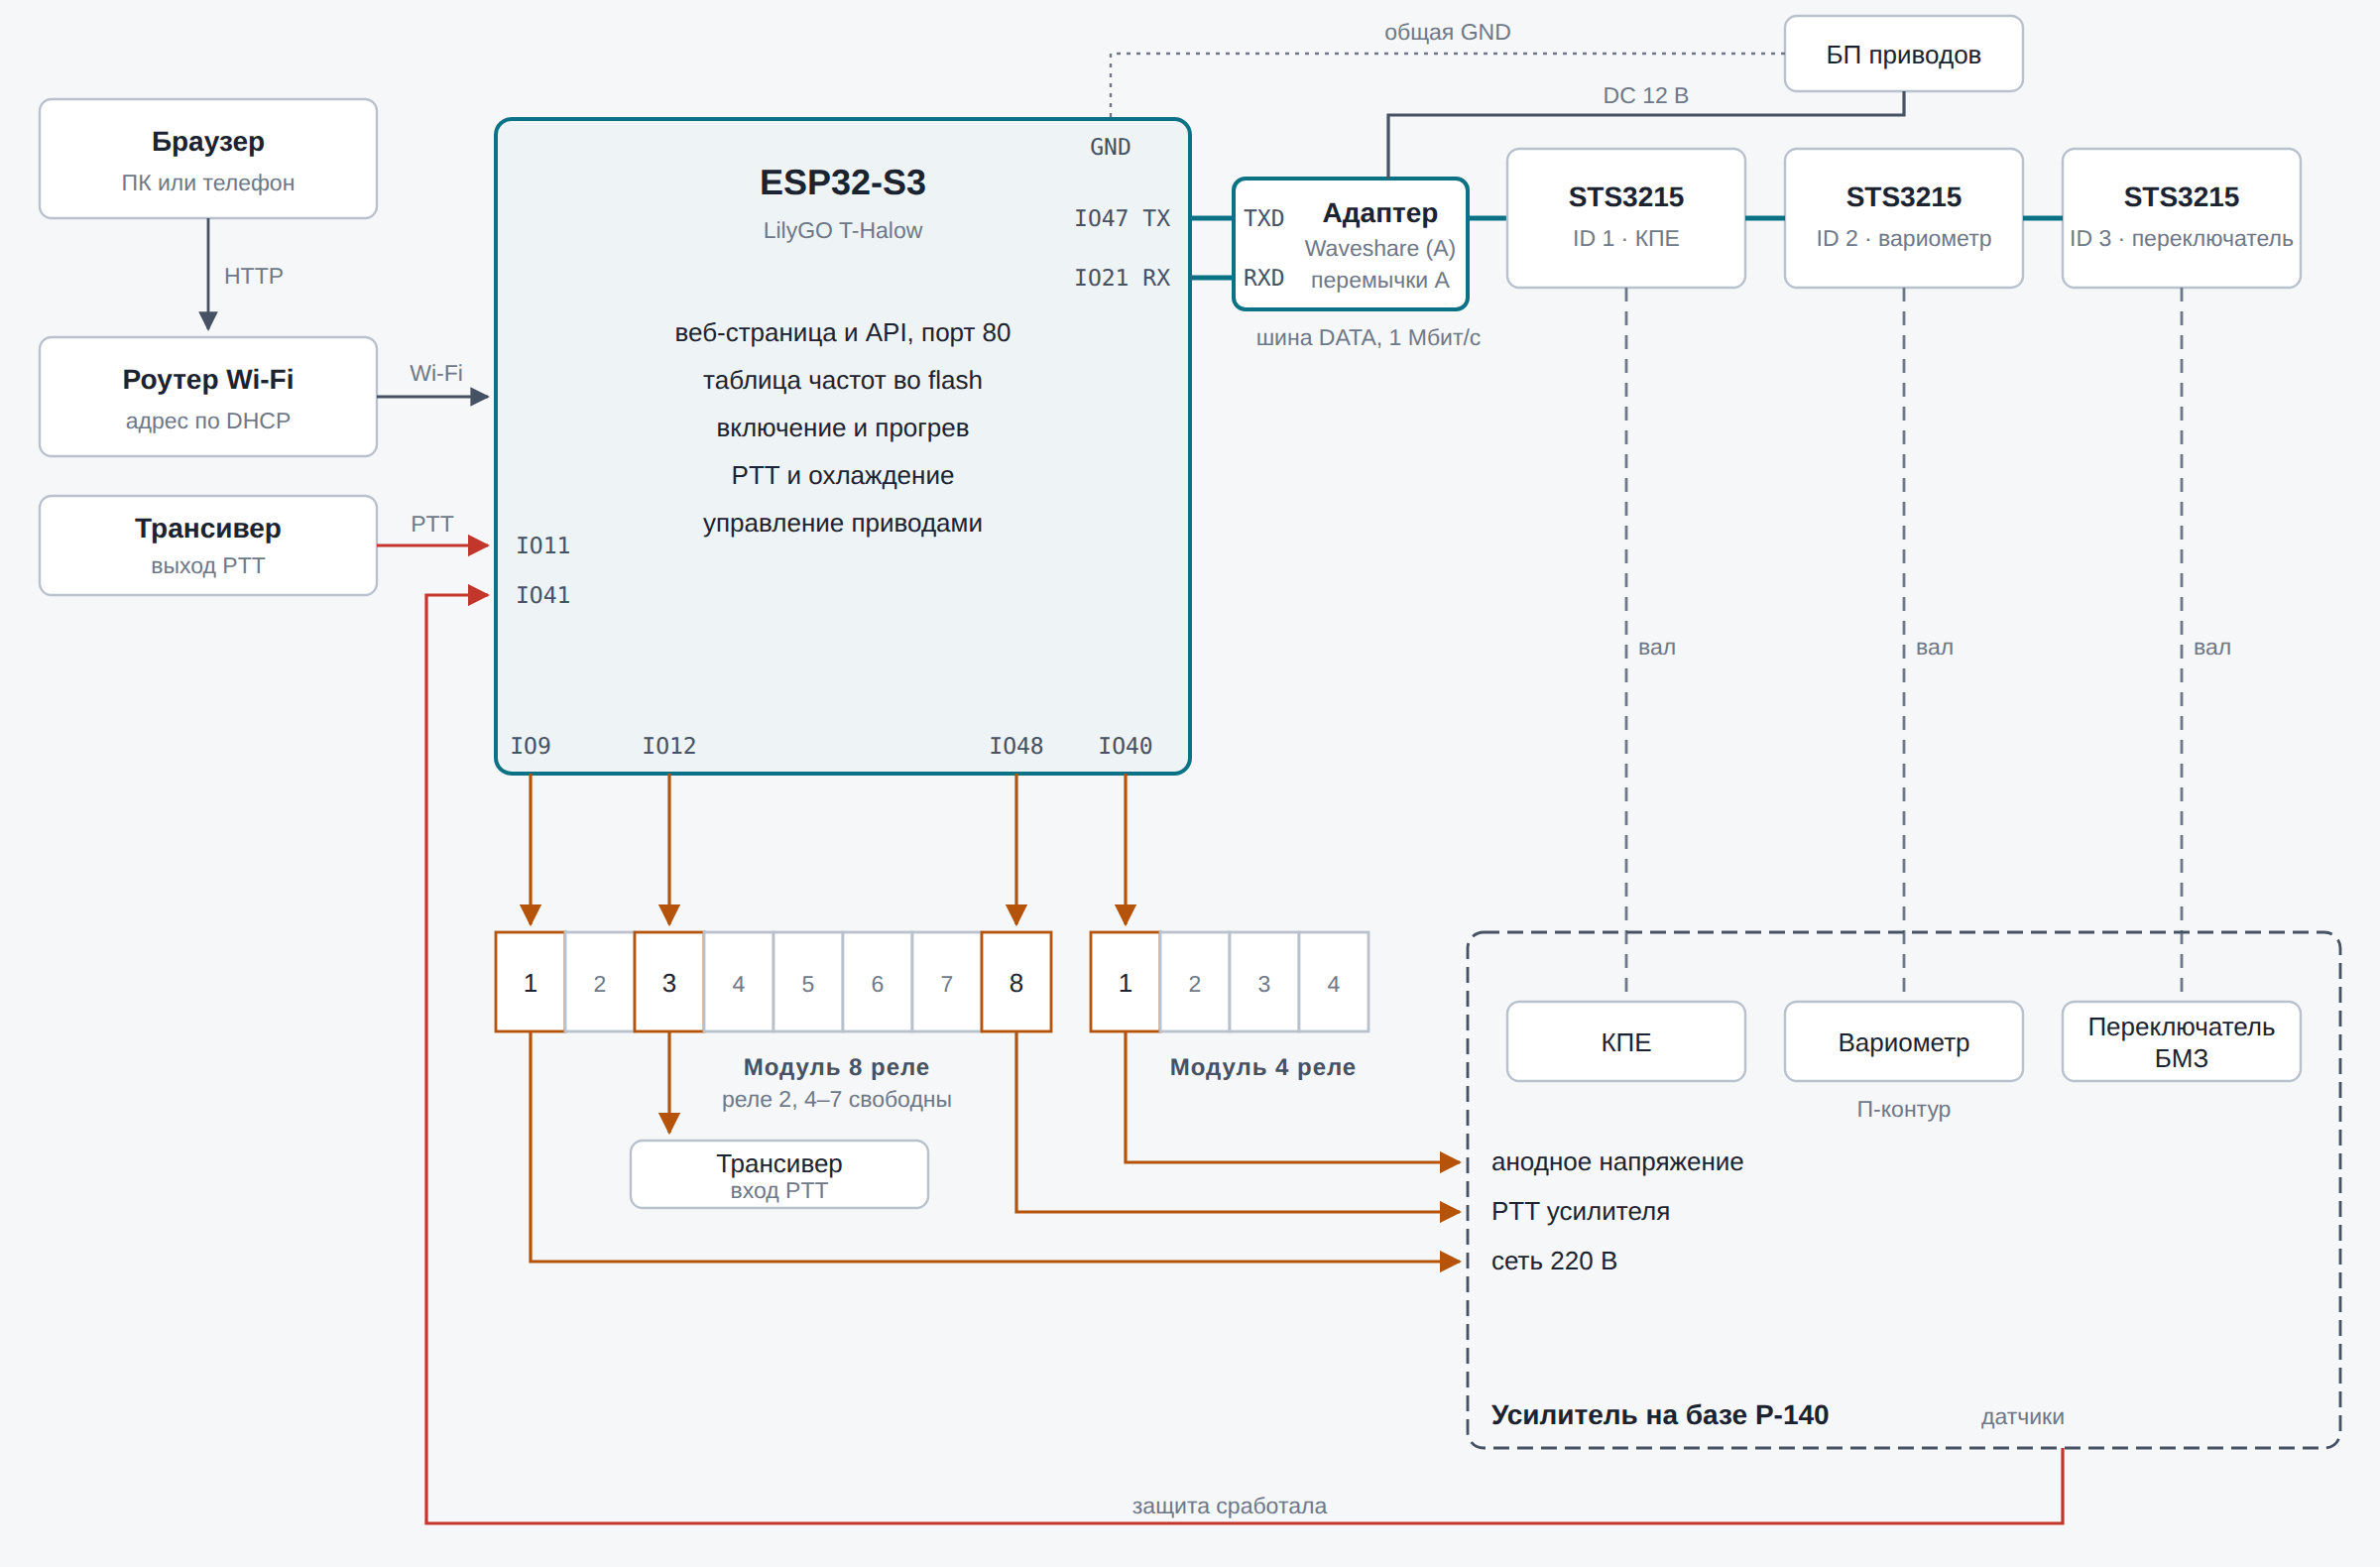
\includegraphics[width=\textwidth]{scheme.png}
  \caption{Общая схема подключения}
\end{figure}

% ---------------------------------------------------------------------------
\section{Безопасность}

\begin{danger}
В усилителе есть \textbf{анодное напряжение} (тысячи вольт) и \textbf{сеть 220~В}.
Подключать контроллер к цепям усилителя можно только при выключенном и отключённом от сети
усилителе, после разряда конденсаторов анодного источника. Если вы не уверены, что умеете
работать с высоким напряжением,~— доверьте подключение к усилителю специалисту.
\end{danger}

\begin{attention}
В текущей версии прошивки для отладки укорочены два времени:
прогрев ламп~— \textbf{10~секунд} вместо 3~минут, охлаждение после передачи~— \textbf{10~секунд}
вместо 5~минут. Перед работой с настоящим усилителем их нужно вернуть
(см. раздел~\ref{sec:timings}). Иначе анодное напряжение подастся на холодные лампы.
\end{attention}

\begin{itemize}
  \item Сервоприводы питаются \textbf{12~В} и только от отдельного блока питания. Никогда не подавайте
        больше 12,6~В: при 14,5~В приводы отказываются работать, а выше 15~В срабатывает защита адаптера.
  \item На входы контроллера (PTT, защита) нельзя подавать напряжение. Их можно только замыкать на «землю»
        (GND) контактом или оптроном.
  \item Пальцы и провода держите подальше от осей во время перестройки: приводы сильные.
\end{itemize}

% ---------------------------------------------------------------------------
\section{Что понадобится}

\subsection{Детали}

Детали можно купить по списку ниже или заказать комплектом: \ordermail.

\noindent\begin{tabularx}{\textwidth}{@{}>{\raggedright\arraybackslash}p{0.58\textwidth}X@{}}
\toprule
\textbf{Деталь} & \textbf{Зачем} \\
\midrule
Плата LilyGO T-Halow (ESP32-S3) & контроллер \\
3 сервопривода Feetech STS3215, \textbf{версия на 12~В} & КПЕ, вариометр, переключатель БМЗ \\
Адаптер Waveshare Bus Servo Adapter (A) & связь с приводами и их питание \\
Блок питания 12~В, не меньше 5~А, штекер 5,5$\times$2,1~мм & питание приводов \\
Модуль на 8 реле с опторазвязкой «для Arduino» & питание усилителя, PTT \\
Модуль на 4 реле & анодное напряжение \\
Блок питания 5~В (зарядка от телефона) и кабель USB-C & питание контроллера \\
Провода «папа-мама» для макетных плат & соединения \\
Муфты или переходники с вала привода на оси усилителя & механика \\
\bottomrule
\end{tabularx}

\subsection{Инструменты}

\begin{itemize}
  \item Компьютер с Linux (для заливки программы в контроллер).
  \item Мультиметр (прозвонка и напряжение).
  \item Домашний роутер с Wi-Fi \textbf{2,4~ГГц} (5~ГГц контроллер не видит).
\end{itemize}

% ---------------------------------------------------------------------------
\section{Сборка}

\subsection{Адаптер шины: перемычки}

На адаптере есть гребёнка из 6 контактов (3 ряда по 2) и две перемычки.
Они выбирают, кто управляет приводами.

\begin{center}
\begin{tabular}{@{}lll@{}}
\toprule
\textbf{Ряд} & \textbf{Контакты} & \textbf{Куда идут} \\
\midrule
Верхний  & RXD, TXD       & разъём UART (к контроллеру) \\
Средний  & U1RXD, U1TXD   & шина приводов \\
Нижний   & CH\_RXD, CH\_TXD & USB-C адаптера (к компьютеру) \\
\bottomrule
\end{tabular}
\end{center}

\begin{itemize}
  \item \textbf{Положение A}~— работа с контроллером: перемычки соединяют \textbf{верхний ряд со средним}.
        Это рабочее положение.
  \item \textbf{Положение B}~— проверка приводов с компьютера через USB-C адаптера: перемычки соединяют
        \textbf{средний ряд с нижним} (см. приложение~\ref{sec:pc}).
\end{itemize}

\begin{hint}
Если не видно, где какой ряд, прозвоните мультиметром: контакты, которые звонятся
на \texttt{TXD} и \texttt{RXD} разъёма UART,~— это верхний ряд.
\end{hint}

\subsection{Адаптер~— контроллер}

Три провода от разъёма UART адаптера к плате T-Halow:

\begin{center}
\begin{tabular}{@{}ll@{}}
\toprule
\textbf{Адаптер} & \textbf{T-Halow} \\
\midrule
TXD & IO47 \\
RXD & IO21 \\
GND & GND \\
\bottomrule
\end{tabular}
\end{center}

\begin{attention}
\textbf{TXD идёт на передачу контроллера, RXD~— на приём}, то есть «TX к TX, RX к RX». Это не ошибка:
подписи на адаптере сделаны со стороны контроллера. Провод GND обязателен.
\end{attention}

\subsection{Сервоприводы}

\begin{enumerate}
  \item Пока \textbf{не подключайте приводы цепочкой}. С завода у всех номер ID~1, и вместе они
        мешают друг другу. Номера назначаются при первом запуске (раздел~\ref{sec:ids}).
  \item У привода два одинаковых разъёма. Приводы соединяются цепочкой: адаптер~— привод~— привод~— привод.
        У адаптера тоже два разъёма, можно подключить две ветки.
  \item Блок питания 12~В~— в разъём DC адаптера (или в винтовую клемму, соблюдая полярность).
        На адаптере загорится красный светодиод.
\end{enumerate}

\begin{verify}
Проверьте наклейку на приводах: напряжение должно быть 12~В. Измерьте напряжение блока питания
мультиметром: 11,5--12,6~В. Блок на 13,8~В (для радиостанций) не подходит.
\end{verify}

\subsection{Реле}

Модули реле включаются \textbf{низким уровнем} (замыканием входа IN на GND). Питание модулей~— 5~В,
земля общая с контроллером.

\begin{center}
\begin{tabular}{@{}lll@{}}
\toprule
\textbf{Модуль, реле} & \textbf{Вывод T-Halow} & \textbf{Что делает} \\
\midrule
8 реле, IN1 & IO9  & включение усилителя (питание) \\
8 реле, IN3 & IO12 & PTT трансивера: передача с веб-страницы \\
8 реле, IN8 & IO48 & PTT усилителя \\
4 реле, IN1 & IO40 & анодное напряжение \\
\bottomrule
\end{tabular}
\end{center}

Остальные реле свободны. Контакты реле (COM/NO) подключаются к соответствующим цепям управления
усилителя и трансивера.

\begin{hint}
Если реле щёлкают неуверенно, снимите перемычку JD-VCC на модуле: питайте вход VCC от 3,3~В
контроллера, а JD-VCC~— от 5~В.
\end{hint}

\subsection{Входы от трансивера и усилителя}

\begin{center}
\begin{tabular}{@{}lll@{}}
\toprule
\textbf{Вывод T-Halow} & \textbf{Сигнал} & \textbf{Как подключить} \\
\midrule
IO11 & PTT от трансивера & выход PTT (SEND) трансивера на IO11, его земля на GND \\
IO41 & сработала защита & контакт или оптрон усилителя между IO41 и GND \\
\bottomrule
\end{tabular}
\end{center}

Вход считается включённым, когда он замкнут на GND. \textbf{Никакого напряжения на эти выводы не подавать.}

\subsection{Питание контроллера}

Плата T-Halow питается через USB-C от блока 5~В или от компьютера. Сначала включайте питание приводов,
потом контроллер (или одновременно).

% ---------------------------------------------------------------------------
\section{Установка программы}

Это делается один раз на компьютере с Linux. Команды вводятся в терминале в папке проекта
\texttt{RemoteTubeAmplifaier}.

\begin{enumerate}
  \item Установите arduino-cli:
\begin{verbatim}
curl -fsSL \
  https://raw.githubusercontent.com/arduino/arduino-cli/master/install.sh \
  | BINDIR=~/.local/bin sh
\end{verbatim}
  \item Установите поддержку ESP32 (ядро версии 3.x):
\begin{verbatim}
~/.local/bin/arduino-cli config add board_manager.additional_urls \
  https://espressif.github.io/arduino-esp32/package_esp32_index.json
~/.local/bin/arduino-cli core update-index
~/.local/bin/arduino-cli core install esp32:esp32
\end{verbatim}
  \item Создайте файл \texttt{esp32-backend/secrets.h} с именем и паролем вашей сети Wi-Fi:
\begin{verbatim}
#pragma once
const char *WIFI_SSID = "имя сети";
const char *WIFI_PASS = "пароль";
\end{verbatim}
  \item Подключите плату к компьютеру кабелем USB-C и залейте программу и веб-страницу одной командой:
\begin{verbatim}
tools/flash.sh
\end{verbatim}
        Скрипт сам соберёт программу, зальёт её и файлы страницы. В конце появится «Готово».
        Если плата не на \texttt{/dev/ttyACM0}, укажите порт: \texttt{tools/flash.sh -p /dev/ttyACM1}.
  \item Узнайте адрес контроллера в сети:
\begin{verbatim}
tools/flash.sh monitor
\end{verbatim}
        Плата пишет адрес при старте: строка вида \texttt{IP: 192.168.0.134}. Если строка уже прошла,
        выйдите из монитора (Ctrl+C), выньте и вставьте кабель USB и снова запустите монитор.
        Ещё проще~— найти устройство \texttt{tubeamp} в списке клиентов роутера.
\end{enumerate}

\begin{hint}
Закрепите этот адрес за платой в настройках роутера (резервирование DHCP), чтобы он не менялся.
\end{hint}

\begin{verify}
Откройте в браузере \texttt{http://<адрес>} (например, \texttt{http://192.168.0.134}).
Должна появиться страница «Ламповый усилитель на базе УМ от Р-140».
\end{verify}

% ---------------------------------------------------------------------------
\section{Первый запуск}

\subsection{Номера (ID) сервоприводов}\label{sec:ids}

Внизу страницы раскройте блок \btn{Сервис: ID сервоприводов}.

\begin{enumerate}
  \item Подключите к адаптеру \textbf{только привод вариометра}. Нажмите \btn{Найти приводы}~—
        появится ID~1 с положением (числом).
  \item В строке «Сменить ID» введите: с \textbf{1} на \textbf{2}, нажмите \btn{Сменить}.
  \item Отключите его. Подключите \textbf{только привод переключателя БМЗ}. Смените ID с \textbf{1} на \textbf{3}.
  \item Привод КПЕ оставьте с ID~1.
  \item Соедините все три привода цепочкой. \btn{Найти приводы} должен показать ID 1, 2 и 3,
        у каждого~— положение.
\end{enumerate}

\begin{attention}
Если в списке ID есть, а положение «$-1$», значит на шине два привода с одинаковым номером.
Отключите лишние и повторите смену номеров.
\end{attention}

\subsection{Ноль переключателя БМЗ}

Положение~1 переключателя~— это ноль привода. Остальные положения идут через $72^\circ$.

\begin{enumerate}
  \item В блоке «Сервис» нажмите \btn{Привести в ноль}. Привод повернётся в ноль.
  \item Ослабьте муфту между приводом и осью переключателя, поставьте переключатель
        \textbf{в положение 1} и затяните муфту, не сдвигая вал привода.
\end{enumerate}

\begin{hint}
Настройка привода переключателя хранится не в нём самом, а в контроллере. Если привод заменить,
достаточно повторить смену ID и этот шаг.
\end{hint}

\subsection{Проверка}

\begin{verify}
Вверху страницы индикаторы «КПЕ», «Вариометр», «Переключатель» должны быть зелёными и показывать числа.
Красный «нет связи»~— см. раздел~\ref{sec:trouble}.
\end{verify}

% ---------------------------------------------------------------------------
\section{Настройка частот}

Таблица частот идёт с шагом 25~кГц по диапазонам 190, 160, 100, 80, 40, 30, 20, 17, 15, 12 и 10~м.
Для каждой частоты нужно один раз подобрать положения приводов.

\begin{enumerate}
  \item Нажмите \btn{Включить} и подтвердите. Дождитесь конца прогрева (обратный отсчёт вверху).
        Пока усилитель выключен или греется, выбирать частоты нельзя.
  \item Включите \btn{Режим настройки}.
  \item Кнопкой диапазона (например, \btn{40m}) откройте диапазон и выберите частоту.
  \item Ползунками и кнопками \btn{$-$100}~\ldots~\btn{+100} подберите КПЕ и вариометр по максимуму
        выходной мощности. Колесо мыши над ползунком~— 10 шагов, с Shift~— 1 шаг.
        В режиме настройки ручки передачу не прерывают: можно настраивать под несущей.
  \item Кнопками \btn{1}~\ldots~\btn{5} выберите положение переключателя БМЗ.
  \item Нажмите \btn{Сохранить}. Частота в таблице получит зелёную полоску.
\end{enumerate}

\btn{Сбросить точку} удаляет настройку выбранной частоты.

\begin{hint}
Сделайте резервную копию: в режиме настройки под таблицей кнопка \btn{Скачать} сохраняет все
настройки в файл. \btn{Загрузить} возвращает их обратно~— например, на новую плату.
\end{hint}

% ---------------------------------------------------------------------------
\section{Работа}

\subsection{Включение}

\begin{enumerate}
  \item Нажмите \btn{Включить}. Усилитель получает питание, начинается прогрев ламп.
  \item После прогрева контроллер сам включает анодное напряжение. Вверху~— «Усилитель включён».
\end{enumerate}

\subsection{Смена частоты}

Выберите частоту в таблице. Приводы поедут в сохранённые положения. На это время передача запрещена,
по окончании разрешается сама.

\subsection{Можно ли передавать}

Под кнопками всегда видна плашка:

\begin{itemize}
  \item \colorbox{tip!20}{Передача разрешена}~— можно работать;
  \item \colorbox{warn!20}{Передача запрещена: \ldots}~— передавать нельзя, после двоеточия причина;
  \item \colorbox{orange!25}{Идёт передача}~— усилитель на передаче.
\end{itemize}

\begin{center}
\noindent\begin{tabularx}{\textwidth}{@{}lX@{}}
\toprule
\textbf{Причина запрета} & \textbf{Что делать} \\
\midrule
усилитель выключен & нажать \btn{Включить} \\
идёт прогрев & подождать окончания отсчёта \\
сработала защита & устранить причину, нажать \btn{Сбросить защиту} \\
перестройка КПЕ и вариометра,\newline поворот переключателя БМЗ & подождать секунду-две \\
нет связи с приводом \ldots & проверить кабель привода и питание 12~В \\
\ldots\ не встал в положение & что-то мешает оси; осмотреть механику, выбрать частоту ещё раз \\
\bottomrule
\end{tabularx}
\end{center}

PTT трансивера проходит на усилитель, только когда передача разрешена.
Кнопка \btn{Передача} на странице переводит трансивер на передачу сама (держится до 60~с, пока
открыта страница) и работает только на включённом прогретом усилителе.

\subsection{Выключение}

Нажмите \btn{Выключить}. Если после последней передачи прошло меньше 5 минут, усилитель
не выключится: лампам нужно остыть. Подождите отсчёт охлаждения или, если очень нужно,
нажмите \btn{Выключить без охлаждения}.

\subsection{Если пропало питание}

\begin{itemize}
  \item Пропало всё: после включения контроллер стартует с выключенным усилителем.
        Включите его заново и выберите частоту. Положения приводов не теряются.
  \item Пропало только питание приводов: передача сразу запрещается. Когда питание вернётся,
        приводы сами встанут в положения текущей частоты.
\end{itemize}

% ---------------------------------------------------------------------------
\section{Если что-то не работает}\label{sec:trouble}

\begin{center}
\noindent\begin{tabularx}{\textwidth}{@{}>{\raggedright}p{0.32\textwidth}X@{}}
\toprule
\textbf{Признак} & \textbf{Что проверить} \\
\midrule
Страница не открывается &
Контроллер включён? Wi-Fi 2,4~ГГц, верные имя и пароль в \texttt{secrets.h}? Адрес не сменился
(посмотреть в мониторе порта)? \\
\addlinespace
\btn{Найти приводы} ничего не находит &
Перемычки адаптера в положении A? Горит красный светодиод адаптера? TXD на IO47, RXD на IO21, GND
подключён? Если всё верно~— поменяйте местами провода TXD и RXD. \\
\addlinespace
Приводы есть, но положение «$-1$» & На шине одинаковые ID~— раздел~\ref{sec:ids}. \\
\addlinespace
Приводы не крутятся, «не встал» &
Напряжение питания 12~В (не 13,8--14,5~В)? Не упирается ли механика? \\
\addlinespace
Красная плашка про версию &
Прошивка и файлы страницы разных версий: залейте всё вместе командой \texttt{tools/flash.sh}. \\
\addlinespace
Реле щёлкают неуверенно & См. подсказку про JD-VCC в разделе «Реле». \\
\bottomrule
\end{tabularx}
\end{center}

% ---------------------------------------------------------------------------
\section{Время прогрева и охлаждения}\label{sec:timings}

В файле \texttt{esp32-backend/esp32-backend.ino} в начале есть строки:
\begin{verbatim}
const uint32_t COOLDOWN_MS = 10000;  // ОТЛАДКА: в усилителе 300000 (5 мин)
const uint32_t WARMUP_MS = 10000;    // ОТЛАДКА: в усилителе 180000 (3 мин)
\end{verbatim}
Для работы с усилителем замените числа: \texttt{COOLDOWN\_MS = 300000} (5 минут),
\texttt{WARMUP\_MS = 180000} (3 минуты), затем залейте программу командой \texttt{tools/flash.sh}.

% ---------------------------------------------------------------------------
\appendix
\section{Проверка приводов с компьютера}\label{sec:pc}

Если контроллер не видит приводы, их можно проверить напрямую с компьютера.

\begin{enumerate}
  \item Перемычки адаптера~— в положение \textbf{B}.
  \item USB-C адаптера~— к компьютеру, питание 12~В включено.
  \item В папке проекта:
\begin{verbatim}
tools/sts-servo.py scan          # найти приводы
tools/sts-servo.py regs 3        # режим, напряжение, температура привода ID 3
tools/sts-servo.py goto 2 1000   # повернуть привод ID 2 в положение 1000
\end{verbatim}
  \item После проверки верните перемычки в положение \textbf{A}.
\end{enumerate}

Нужен Python 3 с пакетом pyserial (\texttt{pip install pyserial}).

\section{Выводы контроллера}

\begin{center}
\begin{tabular}{@{}ll@{}}
\toprule
\textbf{Вывод T-Halow} & \textbf{Назначение} \\
\midrule
IO9  & реле 1 (модуль 8 реле): включение усилителя \\
IO12 & реле 3: PTT трансивера (передача с веб-страницы) \\
IO48 & реле 8: PTT усилителя \\
IO40 & реле 1 (модуль 4 реле): анодное напряжение \\
IO11 & вход PTT от трансивера (замыкание на GND) \\
IO41 & вход «сработала защита» (замыкание на GND) \\
IO47 & шина приводов, передача (на TXD адаптера) \\
IO21 & шина приводов, приём (на RXD адаптера) \\
\bottomrule
\end{tabular}
\end{center}

\end{document}
